% ===================================================================================================
%                                                 |                                                 |
%                                                 |                                                 |
% -------------------------------------------- SECTION ---------------------------------------------|
%                                                 |                                                 |
%                                                 |                                                 |
% ===================================================================================================

\section{Energy and time requirements of the learning process}\label{sec:energy_time_and_power_per_episode}

% % ---
% \begin{figure*}[h!]
% 	\centering%\section{Materials and Methods}\label{sec:materials_and_methods}
% 	\hspace*{\fill}
% 	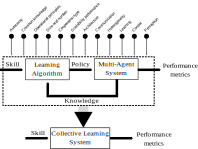
\includegraphics[width=14cm]{closed_loop_collective_dynamics.png}% ===================================================================================================
% 	\hspace*{\fill}%\subsection{Episodic energy and time requirements}\label{sec:power_per_episode}
% 	\caption[] {\label{fig:collective_learning_system} \textbf{A \acl{cl} system.} {A multi-agent system with appropriate learning algorithm(s) and inter-agent knowledge sharing can learn a universe of skills exponentially fast, as reflected by the exponential collection of the knowledge required to learn the skills.}\pending{Consider sending this figure to the supplementary materials.}}% ---
% \end{figure*}


For the discussion in the \nameref{sec:methods}, we relied on our assumption about the duration and energy consumption of a trial episode. In this section, we provide more details about this assumption.
% ---
\begin{figure}[!h]
    \centering
	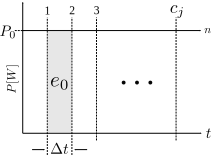
\includegraphics[width=0.45\textwidth]{fig/power_per_episode.png}
	\caption{\textbf{Power consumption per episode.} An episode is an attempt to accomplish a skill. For simplicity, the power to complete an episode is assumed constant.}	
	\label{fig:power_per_episode}
\end{figure}
% ---
\paragraph{Energy requirements}
Under Asm.~\ref{assumption:power_and_episode_time}, the energy consumption of the $n$-th episode $e_j(n)$ is the constant product
% ---
\begin{equation}\label{eq:energy_per_episode}
	e_j(n) = \underbrace{P_0 \: \Delta t}_{\text{constant}} = e_0.
\end{equation}
% ---
Consequently, the energy consumed by a robot learning a skill $ s_j $ is directly proportional to the skill complexity $c_j$; i.e.
% ---
\begin{equation}\label{eq:energy_per_skill}
	E_j =\sum_{n=1}^{c_j} e_j(n) = e_0\:c_j,
\end{equation}
% ---
with $P_0$ being the assumed-constant power to complete an episode, see Fig.~\label{fig:power_per_episode}. The energy spent on learning the universe of skills $\mathcal{S}$ under the absence of knowledge sharing is
% ---
\begin{equation}\label{eq:total_energy}
	E_{\mathcal{S}} = \sum_{j=1}^{{N_{\mathcal{S}}}} E_j = e_0 \:\sum_{j=1}^{{N_{\mathcal{S}}}} c_j%N_{\mathcal{T}} \cdot e_0 \cdot c_j 
\end{equation}
% ---
% ---------------------------------------------------------------------------------------------------
\paragraph{Time requirement} Similarly, the total learning time $T_{\mathcal{S}}$ for a simple agent is
% ---
\begin{equation}\label{eq:total_time}
	T_{\mathcal{S}} = \Delta t \: \sum_{j=1}^{{N_{\mathcal{S}}}} c_j.
\end{equation}
% ---

% ===================================================================================================
%                                                 |                                                 |
%                                                 |                                                 |
% -------------------------------------------- SECTION ---------------------------------------------|
%                                                 |                                                 |
%                                                 |                                                 |
% ===================================================================================================
\newpage
\section{The conventional learning paradigms}\label{sec:conventional_learning_paradigms}

Here we present the detailed derivation of the knowledge acquisition dynamics for \acl{isl}, \acl{il}, \acl{tl}, and \acl{til}. Starting from the generic remaining knowledge model introduced in the \nameref{sec:methods}, we formalize how intra-cluster and inter-cluster similarity, skill memory, and transferability coefficients shape the learning rate in each paradigm. This mathematical groundwork serves as a baseline for contrasting these paradigms with the \acl{cl} formulation in the \nameref{sec:main_results}.

% ---------------------------------------------------------------------------------------------------
\subsection{\Acl{isl}} The $i$-th robot performs \ac{isl} when it learns each skill in the skill universe $\mathcal{S}$ one after another from the ground up, disregarding the accumulating knowledge from already learned skills. In such a case the rate of convergence and the initial remaining knowledge for all skills are given by
% ---		
\begin{subequations}\label{eq:fg_isolated}
	\begin{alignat}{2}
		f_{i,j}\left(\cdot \right) &=  -\alpha_i \\
		g_{i,j}\left(\cdot \right) &= 1,
	\end{alignat}
\end{subequations}
% ---
where $ \alpha>0$ models the rate at which a robot in isolation learns any given skill. Relying on Asm.~\ref{assumption:agent_similarity} we can assign a value to $\alpha$ by using the fundamental complexity $c_0$ as follows
% ---
\begin{equation}\label{eq:isolated_learning_rate}
	\alpha = -\frac{1}{c_0}\text{log}(\epsilon).
\end{equation}
% ---
Since in \ac{isl} the complexity to learn each skill $c^{(\text{IsL})}_{i,j} = c_0$, the trial episodes required by one single robot to learn the skills in a cluster $\mathcal{Z}_k$ is given by
% ---
\begin{equation}
	C^{(\text{IsL})}_{k} = \sum_{j=1}^{N_{\mathcal{Z}}} c^{(\text{IsL})}_{i,j}= N_{\mathcal{Z}}  c^{(\text{IsL})}_{i,j} = N_{\mathcal{Z}} c_0.
\end{equation}
%-- 
Similarly, the total trial episodes to learn the universe of skills is simply
% ---
\begin{equation}
	C^{(\text{IsL})}_{\mathcal{S}} = N_\mathcal{K} N_{\mathcal{Z}} c_0.
\end{equation}
% ---

\textbf{Multi agent case.} Suppose that a batch of $m$ robots is used to learn the same number of skills in parallel in a given cluster $\mathcal{Z}_k$. Such a strategy only distributes equally the total number of episodes by the number of available robots; i.e.
% ---
\begin{equation}
	^{\lvert \lvert}C^{(\text{IsL})}_k=  \overbrace{\frac{1}{m}C^{(\text{IsL})}_k}^{\text{episodes per robot}}.
\end{equation}
% ---

% ---------------------------------------------------------------------------------------------------
\subsection{\textbf{\Acl{il}}}
It corresponds to the continuous aggregation and exchange of knowledge from \emph{intra-cluster} skills. Referring back to Asm.~\ref{assumption:skill_clustering}, the knowledge from skills belonging to a cluster ${\mathcal{Z}_k}$ can be leveraged by an  $i$ in virtue of their significant similarity. As depicted in Fig.~\ref{fig:learning_paradigms_conceptual_figure}~\textbf{A}, a robot ($r_1$ in this case) learns every skill in $\mathcal{Z}_1$ with a rate $\alpha_i$---the self loops---but also retains and uses the acquired knowledge to learn subsequent skills. The effect of \ac{il} on the knowledge collection rate of skill $s_j$ can be modeled to be directly proportional to the number of learned skills $\kappa$ as
% ---
\begin{equation}\label{eq:f_function_incremental}
	f_{i,j}\left(\kappa\right) = -\alpha_i \left(\eta \kappa_i + 1 \right), 
\end{equation}
% ---
where $\eta_i>0$ represents the efficiency of knowledge exchange from the subcluster of learned skills $\zeta_k$ to $s_{j}$.~Different potential models might be used to model the depletion of the initial remaining knowledge represented by $g_{i,j}\left(\kappa\right)$, e.g. a linear decay rate, our expectation is that, under the assumption that a learning strategy involving the ordering of skills according to similarity and their balanced distribution in the different clusters, $g_{i,j}\left(\kappa\right)$ might naturally resemble an exponential decay that is strongly dependent on $\kappa$. Such considerations motivate our choice of the following function
% ---
\begin{equation}\label{eq:g_function_incremental}
	g_{i,j}\left(\kappa\right) = e^{-\delta \kappa},
\end{equation}
%---
again with a factor $\delta>0$ controlling the rate at which the exponential converges. Similar to $\alpha$, using Asm.~\ref{assumption:cluster_size} $\delta$ can be defined as 
% ---
\begin{equation}\label{eq:delta}
	\delta = -\frac{1}{N_\mathcal{Z}}\text{log}(\epsilon).
\end{equation}
% ---
Essentially, such choice of $\delta$ implies that the remaining knowledge in a cluster after seeing all its skills is negligible. Via the exchange factors $(\eta,\delta)$, and since, ideally, if each skill has been successfully learned $\kappa =N_{\zeta_k}$; in \ac{il} the knowledge about every new skill gets gradually increased by leveraging previous knowledge, resulting in
% ---
\begin{equation*}\label{eq:remaining_knowledge__IL}
	\bar{\sigma}^{(\text{IL})}_{i,j}(n) = e^{-\alpha_i  \left(\eta_i N_{\zeta_k}+1\right) n} e^{-\delta N_{\zeta_k}}.
\end{equation*}
% ---
As the complexity $c_{j}$ of a skill can also be interpreted as the number of trial episodes required for the remaining knowledge to go below a threshold $\epsilon$; i.e.
% ---
\begin{equation*}
	\bar{\sigma}^{(\text{IL})}_{i,j}(n) \Big \rvert_{n \ge c^{(\text{IL})}_{j}} \leq \epsilon.
\end{equation*}
% ---
Then, under this scheme the complexity $c^{(\text{IL})}_{j}$ to learn a new is skill in the cluster results in
% ---
\begin{equation}\label{eq:complexity_IL}
	c^{(\text{IL})}_{j} = -\frac{\text{log}(\epsilon) - \text{log}\left(\bar{\sigma}^{(IL)}_{i,j}(0)\right)}{\alpha_i (\eta_i N_{\zeta_k}+ 1)} = -\frac{\text{log}(\epsilon) + \delta N_{\zeta_k}}{\alpha (\eta_i N_{\zeta_k}+ 1)}  .
\end{equation}
% ---
The total number of trial episodes $ C_k $ that an agent following an incremental learning strategy needs to learn the $N_{\mathcal{Z}_k}$ skills in a cluster $ \mathcal{Z}_k $ is given by
% ---
\begin{align}\label{eq:total_episodes_incremental}
	\begin{split}
		C^{(\text{IL})}_k &= \sum^{N_{\mathcal{Z}}}_{j=1} c^{(\text{IL})}_{j}.
	\end{split}
\end{align}
% ---

\textbf{Multi-agent case.} If $m$ robots are used in parallel to divide the load of learning the tasks then
% ---
\begin{align}
	\begin{split}
		{}^{\lvert \rvert}C^{(\text{IL})}_k &= \sum^{\frac{N_{\mathcal{Z}}}{m}}_{j=1} c^{(\text{IL})}_{j}.
	\end{split}
\end{align}
% --
In essence, using $m$ robots without exchanging knowledge only subdivides the learning in every cluster into $m$ smaller problems \emph{without adding any additional benefit to the rate at which knowledge is acquired}. 

% ---------------------------------------------------------------------------------------------------
\subsection{\textbf{Transfer + Incremental Learning (TIL)}}
\Acl{tl} alone refers to the one-time \emph{inter-cluster} exchange of knowledge. Considering $\mathcal{K} = \{ \mathcal{Z}_k \}^{N_\mathcal{K}}_{k=1}$ to be the set of all available skill clusters, \ac{tl} represents the exchange of knowledge from agent $i$'s in-memory learned skills from different \emph{origin} clusters $\mathcal{O} = \{ \mathcal{Z}_1,\mathcal{Z}_2,\ldots,\mathcal{Z}_{k-1} \}$ to the skills that will be learned in a \emph{destination} cluster $\mathcal{Z}_k$ (see Fig.~\ref{fig:learning_paradigms_conceptual_figure}~\textbf{B}). 

Concretely, the effect that \ac{tl} has on the skills of the destination cluster is the reduction of the initial remaining knowledge and the increase of the initial learning rate for all the skills in the target cluster through transferable knowledge fraction factor $\xi_k \in [0,1)$---defined in Eq.~\ref{eq:scaled_transferable_knowledge_fraction}; that is
% ---
\begin{equation}\label{eq:f_function_transfer}
	f_{i,j}\left(N_{\zeta_k}\right) = -\alpha_i\:\left( \frac{\eta_i N_{\zeta_k} + 1}{1 - \xi_{i,j}(\cdot)} \right),
\end{equation}
% ---
and
% ---
\begin{equation}\label{eq:g_function_transfer}
	g_{i,j}\left(N_{\zeta_k}\right) = (1-\xi_{i,j})\:e^{-\delta N_{\zeta_k}}.
\end{equation}
%---

% In essence, $\beta_k$ is the head start granted by knowledge transfer from other clusters to the skills in $\mathcal{Z}_k$. We argue that  $0<\beta_{k} < 1$ since it represents the \emph{aggregated} knowledge exchange factor from the different origin clusters $\mathcal{Z}_{c}$ to the target cluster $\mathcal{Z}_{k}$. Let $0<\beta_{c} < 1$ be the transfer contribution factor of a single origin cluster $\mathcal{Z}_c$. Additionally, consider that
% % ---
% \begin{equation}
% 	\sum\limits_{c=1}^{N_\mathcal{K}}\beta_{c} \leq 1,
% \end{equation}
% % --
% as $1$ represents all the knowledge in $\mathcal{S}$. Asm.~\ref{assumption:cluster_transferability} implies that $\beta_c$ is equal for all the clusters. In this work we select $\beta_c = 1/N_\mathcal{K}$ for simplicity. The aggregated transfer factor $\beta_k$ is the sum of the individual factors from the already-visited clusters; i.e.
% % ---
% \begin{equation}\label{eq:beta_k_transfer}
% 	\beta_{k}= \left(k-1\right)\beta_c = \left(k-1\right)\frac{1}{N_\mathcal{K}}.
% \end{equation}
% % ---

Consequently, the remaining knowledge when transfer and incremental learning are used in conjunction is
% ---
\begin{equation}\label{eq:remaining_knowledge__ITL}
	\bar{\sigma}^{(\text{TIL})}_{i,j}(n) = \left(1- \xi_{i,j}(\cdot) \right)\: e^{-\alpha_i \: \left(\frac{ \eta_i N_{\zeta_k}+1}{1 - \xi_{i,j}(\cdot)}\right) \:n} e^{-\delta N_{\zeta_k}}.
\end{equation}
% ---
Similar to incremental learning, the complexity to learn a skill in transfer learning is
\begin{equation}\label{eq:skill_complexity_TL}
	c^{(\text{TIL})}_{j} = -\frac{1 - \xi_{i,j}(\cdot)}{\alpha_i\: (\eta_i N_{\zeta_k}+ 1)}\:\left[\text{log}(\epsilon) + \delta N_{\zeta_k} - \text{log}(1 - \xi_{i,j}(\cdot))\right]
\end{equation}
% ---
and the total number of episodes  $ C_k $ that an agent requires to learn the $N_{\mathcal{Z}_k}$ skills is merely their sum
% ---
\begin{align}\label{eq:total_episodes_transfer}
	\begin{split}
		C^{(\text{TIL})}_k &= \sum^{N_{\mathcal{Z}}}_{j=1} c^{(\text{TIL})}_{j}.
	\end{split}
\end{align}
% --- 

\textbf{Multi-agent case.} If $m$ robots are used in parallel to divide the load of learning the tasks then, the transfer of knowledge from cluster to cluster is also divided by the number of robots, This implies that the total number of episodes to learn the skills in a cluster is
% ---
\begin{align}
	\begin{split}
		{}^{\lvert \rvert}C^{(\text{TIL})}_k &= \sum^{\frac{N_{\mathcal{Z}}}{m}}_{j=1} c^{(\text{TIL})}_{j}.
	\end{split}
\end{align}
% ---
This case is depicted on Fig.~\ref{fig:learning_paradigms_conceptual_figure}~\textbf{B}, where two robots $ r_1$ and $r_2$ learn skills in four different clusters. The shaded areas are the subclusters of skills learned by each robot. Since they do not share knowledge between them, each robot has access only to the knowledge it has collected and cannot benefit from one another. 


% ===================================================================================================
%                                                 |                                                 |
%                                                 |                                                 |
% -------------------------------------------- SECTION ---------------------------------------------|
%                                                 |                                                 |
%                                                 |                                                 |
% ===================================================================================================
\newpage
\section{Definition comparison between the learning paradigms}
The conceptual distinction between our framework and the conventional understanding of incremental and transfer learning in the machine learning community is summarized in Table~\ref{tab:IL_TL}. While standard approaches emphasize procedural aspects such as sequential model updates and domain adaptation, our formulation reinterprets these paradigms structurally, in terms of how knowledge is reused within and across skill clusters. This comparison clarifies the progressive transition from isolated learning to collective learning as a continuum of knowledge reuse and integration.

\begin{table}[ht]
    \centering
    \scriptsize % reduces font size to ~10 pt
    \renewcommand{\arraystretch}{1.3}
    \caption{Incremental vs.\ Transfer Learning in the ML Community vs.\ Our Framework}
    \label{tab:IL_TL}
    \begin{adjustbox}{width=\textwidth}
        \begin{tabularx}{\textwidth}{lXX}
            \toprule
            \textbf{Concept} & \textbf{ML Research Community (Standard Use)} & \textbf{In Our Framework} \\
            \midrule
            \textbf{Incremental Learning (IL)} &
            Continual or lifelong learning; models are updated sequentially with new data or tasks. The focus is on preventing catastrophic forgetting. &
            \textit{Intra-cluster reuse.} Knowledge from similar skills within the same cluster accelerates learning. Learning rate scales with $\eta_i(\kappa+1)$, depending on the number of already learned skills. \\
            \addlinespace
            \textbf{Transfer Learning (TL)} &
            Knowledge reuse from a source domain or task to a related target, typically via pretraining and fine-tuning. &
            \textit{Inter-cluster reuse.} Transferable fractions $\xi_k, \bar{\xi}_k$ weighted by the similarity matrix $\bm{B}$ govern how knowledge moves across clusters, reducing initial remaining knowledge and accelerating cross-cluster acquisition. \\
            \addlinespace
            \textbf{Combined (TIL)} &
            Not a standard category; sometimes refers to sequential transfer or multitask learning. &
            \textit{Transfer with incremental learning.} Exploits both intra-cluster and inter-cluster reuse. More efficient than IL or TL alone but still lacks inter-agent sharing. \\
            \addlinespace
            \textbf{Collective Learning (CL)} &
            Rarely addressed in mainstream ML beyond federated or swarm approaches. &
            \textit{System-wide accumulation, integration, and composition.} Inter-agent transfer gains $\gamma_{i,l}$ enable horizontal sharing across agents, yielding exponential efficiency and energy gains compared to IL and TL. \\
            \bottomrule
        \end{tabularx}
    \end{adjustbox}
\end{table}


% \textbf{Multi-agent case.} If $m$ robots are used in parallel to divide the load of learning the tasks then, the transfer of knowledge from cluster to cluster is also divided by the number of robots, this implies that \eqref{eq:beta_k_transfer} changes to
% % ---
% \begin{equation}\label{eq:beta_k_transfer_parallel}
% 	{}^{\lvert \rvert}\beta_{k}= \frac{1}{m}\beta_{k}.
% \end{equation}
% % ---
% Correspondingly, when using transfer learning in parallel $\beta_k$ is replaced by ${}^{\lvert \rvert}\beta_{k}$ in \eqref{eq:skill_complexity_TL}. Then, similar to IL, the total number of episodes to learn the skills in a cluster is
% % ---
% \begin{align}
% 	\begin{split}
% 		{}^{\lvert \rvert}C^{(\text{TIL})}_k &= \sum^{\frac{N_{\mathcal{Z}}}{m}}_{j=1} c^{(\text{TIL})}_{j,k}.
% 	\end{split}
% \end{align}
% % ---
% This case is depicted on Fig.~\ref{fig:cluster_to_cluster_knowledge_transfer_parallel}, where two robots $ r_1$ and $r_2$ learn skills in four different clusters. The shaded areas are the subclusters of skills learned by each robot. Since they do not share knowledge between them, each robot has access only to the knowledge it has collected and cannot benefit from one another. 

% ---------------------------------------------------------------------------------------------------
%\subsection*{\textbf{Collective learning (CL)}}
%As mentioned in Sec.~\ref{sec:intro}, EAI agents will be a core element of industrial, healthcare, and domestic ecosystems with advanced communication and remote processing capabilities. Given the anticipated legions of EAI agents executing and learning several different skills at any given time in those environments, it is immediately evident that the previous learning paradigms are not meant to exploit these large number of agents together with the advanced communication and processing infrastructure to take full advantage of the potential for concurrent knowledge exchange among the agents. Therefore, the use of isolated, incremental, and transfer learning by these many agents 
%would directly aggravate computational demand (see challenge C1). As discussed in \cite{Kaelbling2020foundationefficientrobot} an leaning algorithm that would allow an agent to learn new tasks on-the-fly would need to be sample-efficient, generalizable, compositional, and (truly) incremental. Collective learning is the natural paradigm that meets this requirements exploiting the full communication potential of the networked EAI agents to leverage the real-time synergistic exchange and aggregation of collected knowledge to make the learning of tasks energy- and time-efficient.
%
%To formalize this idea, let $ \left\lbrace \rho_i \right\rbrace_{i=1}^{m} $ be a set of robotic agents that defines a community of robots. In collective learning, the different robotic agents $ \rho_i $ develop and accumulate dynamically a common mind (body of knowledge) via networked interactions where individual experience, knowledge and skills are disseminated to all the other elements in the collective. Information flows vertically as previous knowledge is passed on, as well as horizontally by sharing concurrent experience between agents. Via these mechanisms, knowledge can be replicated, complimented and further developed. We take from \cite{Garavan2012CollectiveLearning} two notions central in collective learning that are applicable to the embodied AI agents:
%% ---
%\begin{enumerate}
%	\item Capability to restructure and meet changing conditions
%	\item Aggregation of skills, knowledge, and behaviors
%\end{enumerate}
%% ---
%Collective learning contrasts with the previously discussed incremental learning in that a single agent $ r_i $ can aggregate only so much knowledge via trial and error and is limited by a sequential learning structure. Learning collectively, on the other hand, enforces parallelization of knowledge acquisition via the concurrent learning and sharing of all agents as they acquire new skills, knowledge. Moreover, collective learning involves not only the information acquisition, but also how this information is brought to use to form and develop knowledge. 
%
%CL is not only a promising research direction but, in our opinion, has the potential to be a unifying solution to the grand challenges posed by embodied AI. Furthermore, by incorporating new mechanical designs as elements of the learning pipeline it is possible to iteratively evaluate the energy efficiency of proposed solutions and select the best ones as reference designs for future manufacturing processes with underlying learning, therefore, promoting a cyclical optimization towards a semi-optimal general design.
%
%Unlike isolated and transfer learning, in this paradigm a batch of robots $\left \lbrace r_i \right \rbrace^m_{1}$ not only learn different skills concurrently but also exchange the acquired knowledge between each other and are actually able to leverage it. To enable CL, it is assumed that
%\begin{itemize}
%	\item an inter-agent communication protocol/infrastructure is in place that
%	\item enables agents to concurrently exchange and integrate the self-acquired and received knowledge to
%	\item incrementally speed up the learning of all the agents as a whole.
%\end{itemize}
%% ---
%As a result, the intra- and inter-cluster knowledge transfer is possible. Naturally, the CL paradigm involves a complex scheduling problem to determine the optimal skill distribution and inter-agent knowledge sharing strategy. Since we have not tackled this problem yet, we ground the subsequent discussion on Assumptions~\ref{assumption:average_behavior}, \ref{assumption:agent_similarity},~\ref{assumption:cluster_size}, and~\ref{assumption:cluster_transferability} that suggest an average behavior given a suitable scheduling.
%
%Fig.~\ref{fig:cl_example_figure} illustrates the CL concept, where the self loop represents the dynamics of a single robot learning (at a rate $\alpha$). The exchange of knowledge across agents is represented via the cross-couplings weighted by a parameter $\gamma$ that models how efficient is the bidirectional pairwise knowledge exchange. Similar to transfer learning, if two robots exchange knowledge about skills with low similarity (i.e. skills in different clusters), then $\gamma$ is scaled by the inter-cluster transferability parameter $\beta$. In CL \eqref{eq:simple_knowledge_dynamics} is extended to 
%% ---
%\begin{subequations}\label{eq:collective_knowledge_dynamics}
%	\begin{empheq}[left=\empheqlbrace]{align}
%		\dot{\bar{\bm{\sigma}}}^{(CL)}_{j,k}\left(n\right) &= \left[  f_{j,k}\left(N_{\zeta_k},r\right) \bm{I} + \gamma \bm{A} \odot \bm{B}  \right] \bar{\bm{\sigma}}^{(CL)}_{j,k}\left(n\right)\\
%		\bar{\bm{\sigma}}^{(CL)}_{j,k}(0) &= g_{j,k}\left( N_{\zeta_k}, r\right) \bm{I},
%	\end{empheq}
%\end{subequations}
%% ---
%where $r=m$ is the number of robots that exchange knowledge among them. This implies that now $\bar{\bm{\sigma}}^{}_{j,k} \in \mathbb{R}^r$ is a vector that represents the dynamics of the remaining knowledge of all the $m$ skills being concurrently learned. $\bm{A} \in \mathbb{R}^{r \times r}$ is a zero-diagonal symmetric adjacency matrix whose entry $(\bm{A})_{i,j} = 1$ if robot $i$ exchanges knowledge with robot $j$ and $(\bm{A})_{i,j} = 0$ if it does not. The term $\gamma \in \mathbb{R}_+ $ weighs the knowledge exchange strength among robots. Furthermore, since there may be robots learning skills in different clusters at the same time, the matrix $\bm{B}$, whose entries are $\left(\bm{B}\right)_{i,j} \in \left \lbrace 1, \beta_{k} \right \rbrace$, with
%% ---
%\begin{equation}
%	%\beta_{k} = 1/N_\mathcal{K}, 
%	\beta_{k} = r\frac{ N_{\zeta_k}}{N_\mathcal{S}}, 
%\end{equation}
%% ---
%scales down the knowledge contributions between robots from different clusters. Finally, the operator $\odot$ represents the Hadamard product of matrices. The functions $ f(\cdot)$ and $g(\cdot)$ are now also dependent on the number of robots that exchange knowledge, which directly impacts the number of skills that enter $\zeta_k$ after a learning cycle; i.e.
%% ---
%\begin{equation}\label{eq:f_function_collective}
%	f_{j,k}\left(N_{\zeta_k},r\right) = -\alpha \left( \frac{\eta r N_{\zeta_k} + 1}{1 - \beta_k} \right),
%\end{equation}
%% ---
%and
%% ---
%\begin{equation}\label{eq:g_function_collective}
%	g_{j,k}\left(N_{\zeta_k},r\right) = (1-\beta_k) e^{-\delta r N_{\zeta_k}}.
%\end{equation}
%%---
%Some considerations need to be taken when selecting the value of $\gamma$ given that the dynamics matrix of the collective system
%% ---
%\begin{equation}
%	\bar{\bm{A}}\left(N_{\zeta_k}\right) = f\left(N_{\zeta_k},r\right) \bm{I} + \gamma \bm{A} \odot \bm{B} 
%\end{equation} 
%% ---
%exhibits a dependency on the number of seen skills $N_{\zeta_k}$, which is directly influenced by the number of robots $r$ in the collective. Yet, it can be proven that there is a coupling strength $\gamma$ for a given connectivity $\bm{A}$ that ensures that the remaining knowledge for all skills converges asymptotically to zero.

% ===================================================================================================
%                                                 |                                                 |
%                                                 |                                                 |
% -------------------------------------------- SECTION ---------------------------------------------|
%                                                 |                                                 |
%                                                 |                                                 |
% ===================================================================================================
% ===================================================================================================
% \newpage
% \section{Analysis of the collective learning behavior}\label{sec:collective_learning_analysis}

% \textcolor{blue}{\textbf{THIS TEXT GOES TO SUPPLEMENTARY IN THE STABILITY ANALYSIS}} where the operator $\odot$ represents the Hadamard product of matrices. This expression models $r=m$ robots exchanging knowledge among each other. The vector $\bar{\bm{\sigma}}^{}_{j,k} \in \mathbb{R}^r$ represents the dynamics of the remaining knowledge of all the $m$ skills being concurrently learned. $\bm{A} \in \mathbb{R}^{r \times r}$ is a zero-diagonal symmetric adjacency matrix whose entry $(\bm{A})_{i,j} = 1$ if robot $r_i$ exchanges knowledge with robot $r_j$ and $(\bm{A})_{i,j} = 0$ if it does not.

% $\ldots$ the matrix $\bm{B}$, whose entries are $\left(\bm{B}\right)_{i,j} \in \left \lbrace 1, \beta_{k} \right \rbrace$, $\ldots$

% ===================================================================================================
%                                                 |                                                 |
%                                                 |                                                 |
% -------------------------------------------- SECTION ---------------------------------------------|
%                                                 |                                                 |
%                                                 |                                                 |
% ===================================================================================================
\newpage
\section{\Acl{cl} scenarios}\label{sec:results_supplementaries}

% \subsection{Canonical \ac{cl} scenario}
% \label{sec:canonical_cl_scenario}

% This section provides a detailed description of the idealized simulation framework used to identify the nine canonical \ac{cl} regimes. We specify the scenario structure, parameter ranges, initialization procedures, and classification criteria for the four principal regime types—destructive, canceling, ideal, and compensating. We also discuss how sensitivity analyses were performed to explore the effects of noise, communication delays, and embodiment heterogeneity. 

% \subsubsection{Scenario overview}
% The canonical scenario models an idealized \ac{cl} system in which each of the $N_\mathrm{r}$ \ac{eai} agents in the collective learns a different skill in every learning cycle.\footnote{A learning cycle encompasses all learning episodes required to acquire the skills assigned in that cycle.} This setting emphasizes the role of structured skill distribution and synchronous learning, maximizing opportunities for inter-agent knowledge sharing.

% The skill universe is defined as:
% \begin{equation*}
%     N_\mathcal{S} = 512, \quad N_\mathcal{K} = 4, \quad N_\mathcal{Z} = 128 \; \text{skills per cluster}.
% \end{equation*}
% Skills are grouped into $N_\mathcal{K}$ clusters based on their similarity (recall Fig.~\ref{fig:collective_learning_and_skill_manifold_conceptualization}), enabling both intra-cluster and inter-cluster knowledge reuse. Each skill is represented in the structured skill manifold by its similarity relationships to other skills.

% \subsubsection{Learning and completion criteria}
% The learning dynamics for each skill follow Eq.~\eqref{eq:simple_knowledge_dynamics}, where the remaining knowledge $\bar{\sigma}$ decays as agents accumulate information from:
% \begin{enumerate}
%     \item \emph{Self-learning}: parameterized by the learning gain $\alpha_i$.
%     \item \emph{Intra-cluster retention}: parameterized by $\eta_i$, leveraging previously learned skills in the same cluster.
%     \item \emph{Inter-agent transfer}: parameterized by $\gamma_{i,l}$, capturing knowledge exchanged between agents during concurrent learning.
% \end{enumerate}
% A skill is considered \emph{learned} when the remaining knowledge drops below a fixed threshold:
% \begin{equation*}
%     \bar{\sigma} < \epsilon, \quad \epsilon = 0.01.
% \end{equation*}

% The \emph{fundamental skill complexity}, representing the maximum number of episodes needed to learn a skill in the absence of any prior knowledge or external help, is set to:
% \begin{equation*}
%     c_0 = 100 \quad \text{episodes}.
% \end{equation*}

% \subsubsection{Energy Accounting}
% For simplicity, the energetic cost of each learning episode is assumed constant and denoted $e_0$. This assumption implies that the total learning energy is directly proportional to the total number of episodes required to master all $N_\mathcal{S}$ skills:
% \begin{equation*}
%     E_\mathrm{total} \propto C_\mathrm{total} \times e_0,
% \end{equation*}
% where $C_\mathrm{total}$ is the cumulative episode count across all skills and agents.

% \subsubsection{Parameter Initialization and Sweeps}
% To explore the collective learning regimes, we varied the two principal parameters:
% \begin{itemize}
%     \item \textbf{Intra-agent retention gain} $\bar{\eta}$: average ability of an agent to reuse prior intra-cluster knowledge.
%     \item \textbf{Inter-agent transfer gain} $\bar{\gamma}$: average quality and reliability of knowledge exchange between agents.
% \end{itemize}
% For each regime identification run:
% \begin{align*}
%     \eta_i &\sim \mathcal{N}(\bar{\eta}, \eta_{\Sigma}), \\
%     \gamma_{i,l} &\sim \mathcal{N}(\bar{\gamma}, \gamma_{\Sigma}),
% \end{align*}
% with variances $\eta_{\Sigma}$ and $\gamma_{\Sigma}$ chosen to introduce controlled heterogeneity among agents. Learning gains $\alpha_i$ are drawn from a narrow uniform range $\mathcal{U}(\alpha_\mathrm{min}, \alpha_\mathrm{max})$ to simulate comparable embodiment capabilities.

% \subsubsection{Regime Classification}
% The simulation outcomes are classified into the four principal regimes described in Fig.~\ref{fig:canonical_regimes}:
% \begin{enumerate}
%     \item \textbf{Destructive Regimes}: Robust individual learning undermined by harmful inter-agent exchange ($\bar{\eta} > 0$, $\bar{\gamma} < 0$).
%     \item \textbf{Canceling Regimes}: Mixed interactions where inter-agent transfer partially offsets or degrades individual learning.
%     \item \textbf{Ideal Regimes}: Stable and constructive learning both at the individual and network levels ($\bar{\eta} > 0$, $\bar{\gamma} > 0$).
%     \item \textbf{Compensating Regimes}: Weak individual learning compensated by strong inter-agent knowledge sharing ($\bar{\eta} < 0$, $\bar{\gamma} > 0$).
% \end{enumerate}
% Within each principal regime, we identify the corresponding canonical cases (1–9) based on performance metrics such as success rate, total learning episodes, and stability of acquired knowledge.

% \subsubsection{Additional Analyses}
% We further examine transitional boundaries between regimes, the sensitivity of performance to stochastic variations in $\eta$ and $\gamma$, and the effects of embodiment heterogeneity. These analyses provide insight into the robustness of \ac{cl} across a range of realistic conditions, as discussed in Sec.~\ref{sec:main_results}.


% %########################################################################################################

% \subsection{Smart Factory Scenario: Detailed Description}
% \label{sec:smart_factory_supplement}

% This section expands on the smart factory scenario introduced in the \nameref{sec:main_results}. We provide a structured description covering:
% (i) skill universe construction and cluster structure,
% (ii) product generation process and changeover sequence,
% (iii) parameterization of the power-per-episode calculation,
% (iv) mapping from learning episodes to downtime, and
% (v) sensitivity analysis for different robot-to-skill ratios.
% The aim is to enable readers to replicate or extend this study in their own manufacturing contexts.

% \subsubsection{Scenario Overview}
% We consider a smart factory environment dedicated to the rapid prototyping of advanced smart sensors. The factory comprises flexible, reconfigurable work cells tailored to specific manufacturing processes—e.g., component placement, soldering, assembly, testing, and packaging—allowing rapid adaptation to new tasks and components. Within these cells, robots perform skills such as pick-and-place, gripping and handling, component orientation, precise solder application, optical inspection, force testing, and printed-circuit-board handling.

% \subsubsection{Changeover and Skill Requirements}
% When a new sensor is required (\emph{changeover time}), a new set of skills is needed to manufacture it, leading to a period of production downtime while the \ac{eai} agents learn these skills (see Fig.~\ref{fig:smart_factory_case_study}~\textbf{A}).
% For example:
% \begin{itemize}
%     \item In one shift, product $P_\mathrm{A}$ is manufactured, requiring skills from three clusters: $P_\text{A} \subset \mathcal{Z}_1 \cup \mathcal{Z}_2 \cup \mathcal{Z}_4$.
%     \item At changeover, the next product $P_\mathrm{B}$ requires skills from: $P_\text{B} \subset \mathcal{Z}_1 \cup \mathcal{Z}_3 \cup \mathcal{Z}_4$.
% \end{itemize}
% We assume:
% \begin{enumerate}
%     \item Each new product requires $p$ skills (8 in our case).
%     \item Skills may be repeated across products.
%     \item The number of robots satisfies $N_\mathrm{r} \geq p$.
% \end{enumerate}
% The goal is to determine whether \ac{cl} can minimize the changeover downtime $T_\mathrm{CO}$ by reducing the number of episodes needed to learn the required skills.

% \subsubsection{Power-per-Episode Calculation}
% The power per episode (see Asm.~\ref{assumption:power_and_episode_time}) is defined as:
% \begin{equation}
%     P_0 = P_\text{BEE} + P_\text{MIE} + P_\text{CCE},
% \end{equation}
% where:
% \begin{itemize}
%     \item $P_\text{BEE}$: Basal processes power. We assume $\unit[40]{W}$ per robot, based on state-of-the-art tactile robots~\cite{Kirschner2025CategorizingRB} (see Sec.~\ref{sec:app_cobot_ener_consumption}).
%     \item $P_\text{MIE}$: Motion and interaction power, upper-bounded at $\unit[300]{W}$ for demanding tasks.
%     \item $P_\text{CCE}$: Computation and communication power, assumed to be offloaded to a cloud service. Based on~\cite{Strubell2019EnergyPolicyConsiderations}, we take $\unit[1.42]{kW}$ for a representative machine learning workload.
% \end{itemize}
% With $\Delta t = 60$ seconds per trial episode, these values yield the average energetic demand per episode.

% \subsubsection{Scenario Parameterization}
% The scenario tuple is defined as:
% \begin{equation*}
%     \phi_\text{SF} = \left(N_\mathcal{S}, N_\mathcal{K}, N_\text{r}, \bm{\rho}\right),
% \end{equation*}
% where:
% \begin{itemize}
%     \item $N_\mathcal{S} = 512$: total skills, evenly split into $N_\mathcal{K} = 4$ clusters ($N_\mathcal{Z} = 128$ skills per cluster).
%     \item $c_0 = 100$: fundamental skill complexity (trial episodes).
%     \item $\epsilon = 0.01$: knowledge lower bound.
%     \item $N_\text{r} = 8$: \ac{eai} agents in the collective.
% \end{itemize}
% Agent parameters:
% \begin{itemize}
%     \item Learning gain $\alpha_i \sim \mathcal{U}(\alpha_\text{min}, \alpha_\text{max})$, with $\alpha_\text{max} = 1.5\,\alpha_\text{min}$ and $\alpha_\text{min}$ from Eq.~\eqref{eq:isolated_learning_rate}.
%     \item Knowledge depletion rate $\delta$ from Eq.~\eqref{eq:delta}.
%     \item Intra-cluster gain: They are episodic and taken as $\eta_i(n) \sim \mathcal{N}(\bar{\eta}, \eta_{\Sigma}) \;|\; \bar{\eta} = 0.01, \; \eta_{\Sigma} = 0.1$.
%     \item Inter-agent gain: The entries of matrix $\bm{\Gamma} $ are also episodic and defined by $\gamma_{i,l}(n) \sim \mathcal{N}(\bar{\gamma}, \gamma_{\Sigma}) \;|\; \bar{\gamma} = 0.01, \; \gamma_{\Sigma} = 0.1$.
% \end{itemize}

% \subsubsection{Comparative Analysis}
% Figure~\ref{fig:smart_factory_case_study} presents the results for \ac{isl}, \ac{il}, \ac{til}, and \ac{cl} under the above parameterization. As shown in the main text, \ac{cl} consistently outperforms other paradigms in both episode count and energy efficiency, enabling rapid adaptation to new product requirements and minimizing $T_\mathrm{CO}$.

% \newpage
% \section{Dummys}
\subsection{Canonical \ac{cl} scenario}
\label{sec:canonical_cl_scenario}

This section details the idealized simulation framework used to study the dynamics of a \ac{cl} system and to identify the nine canonical regimes described in \nameref{sec:main_results}. We specify the skill universe, learning setup, parameter ranges, and classification criteria for the four principal regime types---destructive, canceling, ideal, and compensating---and discuss sensitivity analyses on noise, communication delays, and embodiment heterogeneity.

\subsubsection{Scenario overview}
The canonical scenario models an idealized \ac{cl} system in which each of the $N_\mathrm{r}$ \ac{eai} agents learns a different skill in every learning cycle.\footnote{A learning cycle encompasses all learning episodes required to acquire the skills assigned in that cycle.} The skill universe is defined as:
\begin{equation*}
    N_\mathcal{S} = 512, \quad N_\mathcal{K} = 4, \quad N_\mathcal{Z} = 128 \; \text{skills per cluster}.
\end{equation*}
Skills are grouped into $N_\mathcal{K}$ clusters based on similarity metrics (see Fig.~\ref{fig:collective_learning_and_skill_manifold_conceptualization}), allowing both intra-cluster and inter-cluster knowledge reuse.

\subsubsection{Learning dynamics and completion criteria}
The learning dynamics follow Eq.~\eqref{eq:simple_knowledge_dynamics}, where the remaining knowledge $\bar{\sigma}$ decays through:
\begin{enumerate}
    \item \emph{Self-learning} ($\alpha_i$): direct acquisition without external help.
    \item \emph{Intra-cluster retention} ($\eta_i$): reuse of skills from the same cluster.
    \item \emph{Inter-agent transfer} ($\gamma_{i,l}$): exchange of knowledge with peers.
\end{enumerate}
A skill is considered learned when $\bar{\sigma} < \epsilon$, with $\epsilon = 0.01$. The fundamental skill complexity is $c_0 = 100$ episodes, representing the upper bound on trials needed without prior knowledge.

\subsubsection{Energy model}
The energetic cost per learning episode is constant ($e_0$), implying:
\begin{equation*}
    E_\mathrm{total} \propto C_\mathrm{total} \: e_0,
\end{equation*}
where $C_\mathrm{total}$ is the total number of episodes. This links regime performance directly to energy efficiency.

\subsubsection{Parameter initialization and sweeps}
To explore the nine canonical regimes, we varied:
% ---
\begin{itemize}
    \item \textbf{Intra-agent retention gain} $\bar{\eta}$: average intra-cluster reuse ability.
    \item \textbf{Inter-agent transfer gain} $\bar{\gamma}$: average reliability of inter-agent sharing.
\end{itemize}
% ---
For each simulation:
%---
\begin{align*}
    \eta_i(n) &\sim \mathcal{N}(\bar{\eta}, \eta_{\Sigma}) \lvert \bar{\eta} = 0.01, \; \eta_{\Sigma} = 0.1,~\text{and}\\
    \gamma_{i,l}(n) &\sim \mathcal{N}(\bar{\gamma}, \gamma_{\Sigma})|\; \bar{\gamma} = 0.01, \; \gamma_{\Sigma} = 0.1,
\end{align*}
% ---
implying that these parameters change per learning episode $n$. Finallly, we chose $\alpha_i \sim \mathcal{U}(\alpha_\mathrm{min}, \alpha_\mathrm{max})$ from Eq.~\eqref{eq:isolated_learning_rate}, ensuring comparable embodiments, and selected the knowledge depletion rate $\delta$ as per Eq.~\eqref{eq:delta}.

\subsubsection{Regime classification}
Simulations were classified into:
\begin{enumerate}
    \item \textbf{Destructive} ($\bar{\eta} > 0$, $\bar{\gamma} < 0$)
    \item \textbf{Canceling}: partial mutual degradation of learning.
    \item \textbf{Ideal} ($\bar{\eta} > 0$, $\bar{\gamma} > 0$)
    \item \textbf{Compensating} ($\bar{\eta} < 0$, $\bar{\gamma} > 0$)
\end{enumerate}
Each principal regime contains one or more canonical cases (1–9), differentiated by success rate, total episodes, and knowledge stability.

\subsection{Smart factory scenario}
\label{sec:smart_factory_supplement}

We now present a more application-oriented scenario based on the \emph{smart factory} case study in \nameref{sec:main_results}. Here, the emphasis is on skill acquisition under realistic product changeover conditions, linking \ac{cl} performance to downtime and energy consumption.

\subsubsection{Scenario overview}
The smart factory produces advanced smart sensors in flexible, reconfigurable work cells designed for rapid adaptation. Robots execute skills such as pick-and-place, gripping, soldering, inspection, and testing.

\subsubsection{Changeover process and skill requirements}
When production switches to a new sensor, a new set of $p$ skills is required, potentially overlapping with previously learned skills. For example:
\begin{itemize}
    \item $P_\mathrm{A}$: $P_\mathrm{A} \subset \mathcal{Z}_1 \cup \mathcal{Z}_2 \cup \mathcal{Z}_4$
    \item $P_\mathrm{B}$: $P_\mathrm{B} \subset \mathcal{Z}_1 \cup \mathcal{Z}_3 \cup \mathcal{Z}_4$
\end{itemize}
We assume $N_\mathrm{r} \geq p$---with $p=8$ in our case---and study whether \ac{cl} can minimize changeover downtime $T_\mathrm{CO}$ by reducing episodes needed for new skills.

\subsubsection{Power-per-episode calculation}
From Asm.~\ref{assumption:power_and_episode_time}:
\begin{equation}
    P_0 = P_\text{BEE} + P_\text{MIE} + P_\text{CCE}.
\end{equation}
Assumptions:
\begin{itemize}
    \item $P_\text{BEE} = \unit[40]{W}$ (tactile robots~\cite{Kirschner2025CategorizingRB})
    \item $P_\text{MIE} \approx \unit[300]{W}$ (upper bound for demanding tasks)
    \item $P_\text{CCE} \approx \unit[1.42]{kW}$ (cloud-based ML workload~\cite{Strubell2019EnergyPolicyConsiderations})
\end{itemize}
With $\Delta t = 60\ \mathrm{s}$ per episode, $e_0 = P_0 \: \Delta t$.

\subsubsection{Parameterization}
We set:
\begin{itemize}
    \item $N_\mathcal{S} = 512$, $N_\mathcal{K} = 4$, $N_\mathcal{Z} = 128$
    \item $c_0 = 100$, $\epsilon = 0.01$, $N_\mathrm{r} = 8$
    \item $\alpha_i \sim \mathcal{U}(\alpha_\mathrm{min}, 1.5\,\alpha_\mathrm{min})$
    \item $\eta_i(n) \sim \mathcal{N}(0.01, 0.1)$
    \item $\gamma_{i,l}(n) \sim \mathcal{N}(0.01, 0.1)$
\end{itemize}

\subsubsection{Comparative analysis}
Figure~\ref{fig:smart_factory_case_study} compares \ac{isl}, \ac{il}, \ac{til}, and \ac{cl}. In this realistic context, \ac{cl} delivers faster skill acquisition, earlier onset of zero-shot learning, and $\sim$90\% lower energy use than the best conventional paradigm (TIL).



% ===================================================================================================
%                                                 |                                                 |
%                                                 |                                                 |
% -------------------------------------------- SECTION ---------------------------------------------|
%                                                 |                                                 |
%                                                 |                                                 |
% ===================================================================================================
\newpage
\section{Technical data and references}\label{sec:technical_data_and_references}
%In this section, we compile reference data and assumptions used throughout the manuscript to support our arguments.
This section expands on the quantitative data and industry trends underlying the three grand energy challenges (C1–C3) discussed in the main text. We provide extended statistics, historical growth curves, and technical sources for data center energy use, industrial and collaborative robot deployment, and the manufacturing-related energy footprint of AI-capable machines. The intent is to give readers a deeper factual foundation for the scale of the problem and its projected evolution.

% ===================================================================================================
\subsection{World Robot Energy Consumption (WREC) estimation}\label{sec:app_robot_ener_consumption}

% ===================================================================================================
\paragraph{Industrial and cobot installations}\label{sec:robot_statistics}
According to the International Federation of Robotics (IFR) the unit sales of collaborative robots in relation to conventional industrial robots has been constantly increasing in the past years \cite{statista_ir_cobot_share}. Recent data, see Fig.~\ref{fig:industrial_cobot_share}, suggest that cobots now make almost 15~\% of the sales.
%---
\begin{figure}[!h]
	\centering
	\includegraphics[width= 0.45\textwidth]{fig/share_industrial_and_cobots.png} 
	\caption{\textbf{Unit sales share industrial robots to cobots.} Cobots have been steadily gaining representation in the robotics market.}
	\label{fig:industrial_cobot_share}
\end{figure}
% ---

The unit sales are congruent with the the estimated operational stock of industrial (Fig.~\ref{fig:ir_stock}) robots and cobots (\ref{fig:cobot_stock}).
% ---
\begin{figure*}[t!]
	\centering
	\hspace*{\fill}
	\begin{subfigure}[b]{0.45\textwidth}
		\subcaption{}
		\includegraphics[width= \textwidth]{ir_units_projections.png}
		\label{fig:ir_stock}
	\end{subfigure}
	\hfill
	\begin{subfigure}[b]{0.45\textwidth}
		\subcaption{}
		\includegraphics[width= \textwidth]{cb_units_projections.png}
		\label{fig:cobot_stock}
	\end{subfigure}
	\hspace*{\fill}	
	\caption[] {\label{fig:robot_forecasts} \textbf{Forecasts for robot operational stock.} (\subref{fig:ir_stock}) industrial robots install base forecast and (\subref{fig:cobot_stock}) cobots install base forecast.}	
\end{figure*}
% ---


\paragraph{WREC}
To provide estimates of the worldwide energy consumption of industrial and collaborative robots we surveyed various sources including reports from consulting agencies and non-profit organizations, news articles and manufacturer press releases and data-sheets to determine essential data such as the operational stock and power consumption per type of robot.

According to \cite{montaqim2015} and available press releases of different robotic companies \cite{fanuc2015, yaskawa2014, ABB2015}, the approximate distribution of the industrial robot install base per manufacturer is shown in Fig.~\ref{fig:manufacturers_pie}.
% ---
\begin{figure*}[!h]
	\centering
	\hspace*{\fill}
	\begin{subfigure}[t]{0.45\textwidth}
		\subcaption{}
		\includegraphics[width= \textwidth]{manufacturers}
		\label{fig:manufacturers_pie}
	\end{subfigure}
	\hfill
	\begin{subfigure}[t]{0.45\textwidth}
		\subcaption{}
		\includegraphics[width=\textwidth]{industrial_robots_average_power_per_category} \label{fig:ir_average_power}
	\end{subfigure}
	\hspace*{\fill}
	\caption[] {\label{fig:ir_statistics} \textbf{Industrial robots statistics.} (\subref{fig:manufacturers_pie}) Percentage of installed industrial robots per manufacturer and (\subref{fig:ir_average_power}) average power consumption of industrial robots per category.}
\end{figure*}
% ---

Since Fanuc, Yaskawa, and ABB make for two-thirds of the total install base of industrial robots, we took the power consumption of the robots from those manufacturers to estimate the total power consumption. After surveying the data-sheets for the different robot types in their portfolio, the average power consumption for each model was estimated. Additionally, every manufacturer classifies their robots according to one or more possible applications, which can be grouped into the application categories defined by the IFR. The average power consumption was calculated for every application using the values reported in the robot data-sheets. Finally, the power consumption for each category was computed as a weighted average based on the companies' market share percentage (assuming that 68 \% is the total number of robots)\footnote[1]{These numbers should be used with discretion since there is no available information on which are the most common installed robot models. This information may change the estimation.}. The estimated power consumption per robot application is shown in Fig.~\ref{fig:ir_average_power}. Using these numbers and the estimated operational stock of industrial robots reported in \cite{statista_ir_operational_stock} and by the International Federation of Robotics (see Fig.~\ref{fig:ir_stock}), the estimated worldwide industrial robot energy consumption was computed and shown in Fig.~\ref{fig:energy_consumption_trends_ai_and_robotics}.

% ===================================================================================================
% \subsection{External energy statistics (data center, industrial, and service robotics energy consumption)}\label{sec:energy_demands_in_ai_and_robotics}
% ---
\begin{figure*}[h!]
	\centering
	\hspace*{\fill}
	\includegraphics[width=\textwidth]{energy_consumption_trends_ai_and_robotics.png}
	\hspace*{\fill}
	\caption[] {\label{fig:energy_consumption_trends_ai_and_robotics} \textbf{Energy demands in \ac{ai} and robotics.} Global electricity demand of data centers (\textsc{Left}), adapted from \cite{andrae2015global}. The estimated World Robot Energy Consumption of industrial (\textsc{Middle}) and collaborative robots (\textsc{Right}).}
\end{figure*}
% ---

% ===================================================================================================
\subsection{ Representative power specifications for state-of-the-art collaborative robots used in parameter setting}\label{sec:app_cobot_ener_consumption}
%---
\begin{figure}[!h]
	\centering
	\includegraphics[width=0.45\textwidth]{cobot_watt_per_kg.png}
	\caption{\textbf{Power consumption per payload for different cobots.} The average power consumption can be estimated at around 40 W.}
	\label{fig:cobot_watt_per_kg}
\end{figure}
%---
To approximate the energy consumption of cobots we looked at the power consumption per payload of various manufacturers, see Fig.~\ref{fig:cobot_watt_per_kg} resulting in an average power consumption of approximately 40 W. Together with a typical power consumption of the robot controller of 60 W \cite{Heredia2023BreakingEnergyConsumption}, we consider a total of 100 W power demand. Similar to the industrial robots, the worldwide energy consumption was calculated assuming a 24/7 operation.



